\documentclass[11pt, english, fleqn, DIV=15, headinclude]{scrartcl}

\usepackage[bibatend, color]{header}

\usepackage{pdflscape}
\usepackage[section]{placeins}

\hypersetup{
    pdftitle=
}

\newcommand\mpi{m_{\piup}}
\newcommand\mpipi{m_{\piup\piup}}

\subject{physics760 Computational Physics}
\title{Analysis of $\piup$-$\piup$ lattice QCD scattering data}
%\subtitle{}
\author{
    Martin Ueding \\ \small{\href{mailto:mu@martin-ueding.de}{mu@martin-ueding.de}}
}

\begin{document}

\maketitle

\begin{abstract}
    % TODO
\end{abstract}

\tableofcontents

\newpage

\section{Data generation}

\subsection{Metropolis algorithm}

\subsection{Correlation functions}

\section{Analysis methods}

Figure~\ref{fig:analysis-flow} shows the data flow in the analysis. This
section will go through the whole analysis in the order of the flow chart. The
methods used will be explained along the way when they are needed.

\begin{figure}[htbp]
    \centering
    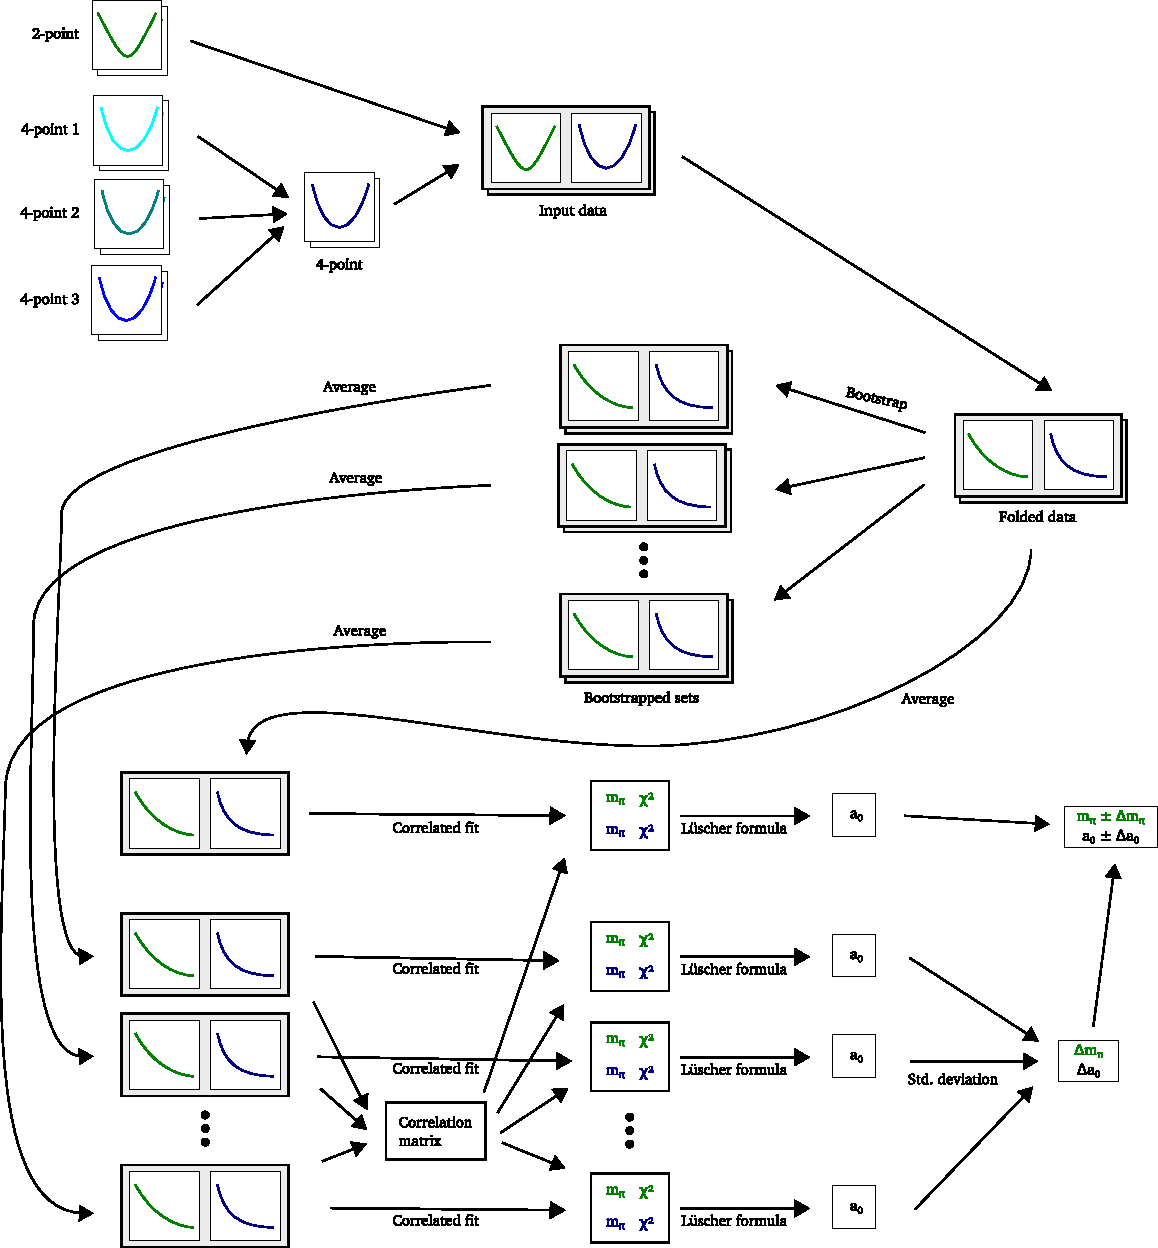
\includegraphics[width=\linewidth]{sketches/Zeichnung.pdf}
    \caption{%
        Data flow in the analysis. The first step is the import of the data,
        which is covered in section~\ref{sec:import}. The two and four point
        functions are combined into pairs for each configuration. The data is
        then folded in half. The bootstrap step is covered in
        section~\ref{sec:bootstrap}. Then a correlated fit is performed, see
        section~\ref{sec:correlated_fit} for details. The second to last step
        is the application of Lüscher's formula, see
        section~\ref{sec:scattering_length}. The results are shown in
        section~\ref{sec:results}.
    }
    \label{fig:analysis-flow}
\end{figure}

\subsection{Import data}
\label{sec:import}

The data that I was given is organized in different ensembles (like A30.32,
A100.24). For each ensembles, multiple configurations were simulated. The
output of each configuration is a two-point correlation function $C_\piup(t)$
and three four-point correlation functions $C_{\piup\piup}^{(i)}(t)$. Those
three different contractions are combined into a single
$\piup\piup$-correlation function:
\begin{equation}
    C_{\piup\piup}(t) = C_{\piup\piup}^{(1)}(t) + C_{\piup\piup}^{(2)}(t)
    - 2 C_{\piup\piup}^{(3)}(t).
\end{equation}

Some of the ensembles had multiple versions of the data in it. I analyzed all
of them sorted by file name. In the tables, you will find the ensembles
multiple times, those are the different versions.

The number of configurations in each ensemble is called $N$.

In both space and time, the lattice used in the computation has periodic
boundary conditions. This leads to a symmetry which $t$ and $T-t$ closely
related. The correlation functions $C(t_1, t_2)$ are symmetric in $t_1$ and
$t_2$, such that only the data in the interval $[0, T/2]$ carries independent
information. Before starting any other calculations with the data, it is folded
in half, like also shown in figure~\ref{fig:folded} later on.

\subsection{Bootstrap}
\label{sec:bootstrap}

All error estimation is done with the bootstrap method. The number of bootstrap
samples $R$ was set to $R = 3N$.

\subsection{Correlated fit}
\label{sec:correlated_fit}

The pion masses are contained in the correlation functions in the form of an
exponential decay constant. Since time is periodic in this simulation, the
correlation function is also periodic with the temporal lattice extent $T$.
Therefore, the expectation is not a simple exponential decay but a cosh-like
function. The four-point functions also have a constant contribution due to the
finite lattice extent. For both two and four point functions, the functions
that I fitted to the folded data are:
\begin{equation}
    \label{eq:fit2}
    m_\piup(t, \lambda) = \lambda_1 \sbr{\exp(-\lambda_2 t) + \exp(-\lambda_2
    [T - t])}
\end{equation}
and
\begin{equation}
    \label{eq:fit4}
    m_{\piup\piup}(t, \lambda) = \lambda_1 \sbr{\exp(-\lambda_2 t) + \exp(-\lambda_2
    [T - t])} + \lambda_3.
\end{equation}

The folded correlation functions with the fit functions are shown in
figure~\ref{fig:folded}.

\begin{figure}[htbp]
    \centering
    \begin{minipage}[c]{0.49\linewidth}
        \centering
        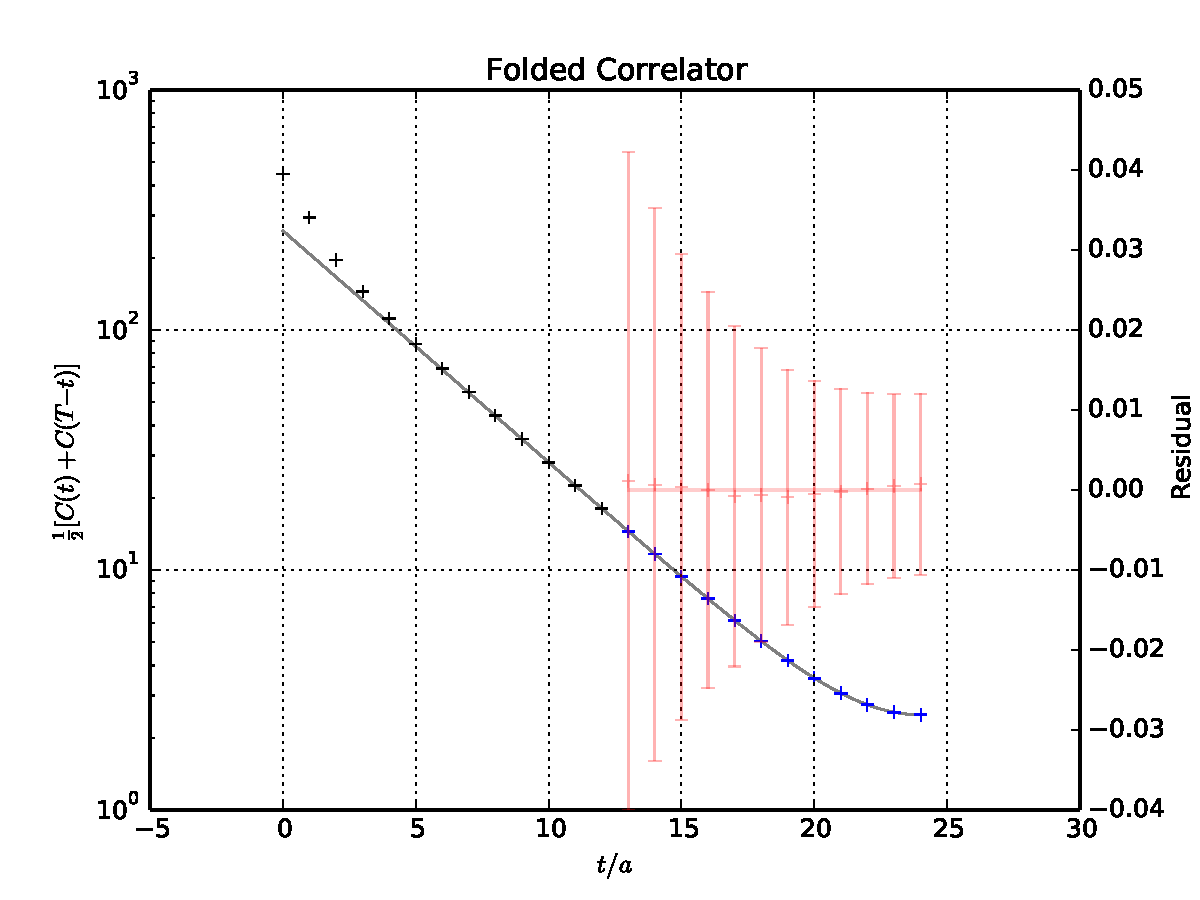
\includegraphics[width=\linewidth]{plots/A100_24_L24_T48_beta190_mul0100_musig150_mudel190_kappa1632550__ev120__TB2_SO_LI6_new_c2_folded.pdf}
    \end{minipage}
    \hfill
    \begin{minipage}[c]{0.49\linewidth}
        \centering
        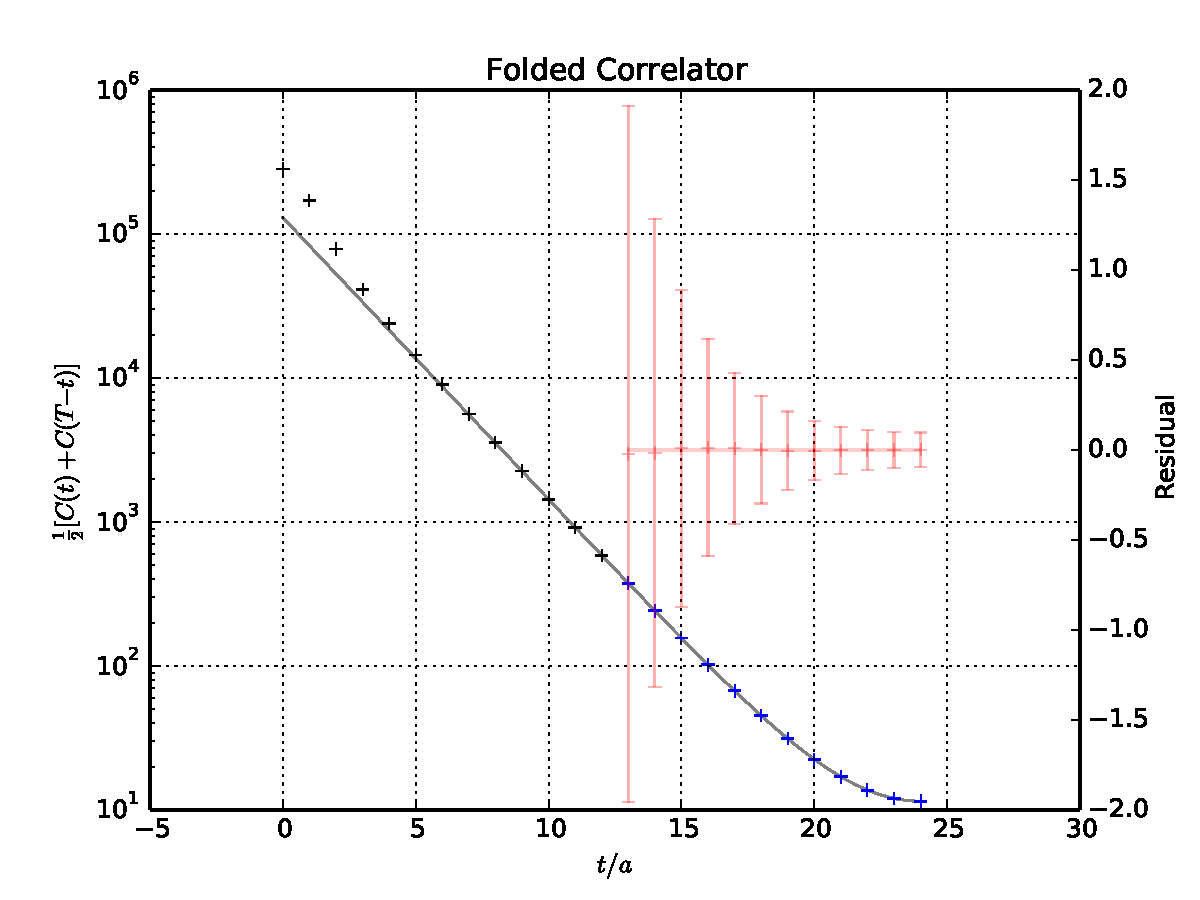
\includegraphics[width=\linewidth]{plots/A100_24_L24_T48_beta190_mul0100_musig150_mudel190_kappa1632550__ev120__TB2_SO_LI6_new_c4_folded.pdf}
    \end{minipage}
    \caption{%
        Folded correlation functions with cosh-like fit function. On the left
        side, the two point function is shown, the four point function on the
        right. Only the blue data points were used for fitting. The right
        ordinate shows the residuals in great magnification (red). One can see
        that the errors seem way too large. This is a result of the
        autocorrelation of the data points.
    }
    \label{fig:folded}
\end{figure}

The correlation functions themselves are highly correlated with respect to
time. Therefore, a regular least squared fit would give a $\chi^2$ that was way
too low. The $p$-values usually end up around 1, which does not imply a perfect
fit but that the data fits the model too \emph{well}.

For the correlated fit, a new likelihood function is needed. I chose to keep
the least squared likelihood function but incorporate the correlation into the
$\chi^2$. First, a correlation matrix $\tens C$ is needed, which is computed
from the $R$ bootstrap samples:
\begin{equation}
    \label{eq:correlation_matrix}
    C_{ij} := \frac{1}{R[R-1]} \sum_{k=1}^R
    [x_{ik} - \bar x_{iR}] [x_{jk} - \bar x_{jR}]
    \eqnsep
    \bar x_{iR} := \frac 1R \sum_{r=1}^R x_{ir}.
\end{equation}

Using this correlation matrix, a new $\chi^2$ can be defined which incorporates
the inverse correlation matrix:
\begin{equation}
    \label{eq:chisq}
    \chi^2_\text{corr} := \sum_{i, j}^T
    \left[ \bar x_{iR} - f(t_i, \lambda) \right]
    C^{-1}_{ij}
    \left[ \bar x_{jR} - f(t_j, \lambda) \right].
\end{equation}
The regular $\chi^2$ has $\tens C^{-1} = \tens 1$ and is just the sum of the
squared residuals.

In the curve fitting process, a function like
\texttt{scipy.optimize.curve\_fit} tries to find the parameters $\lambda$ such
that $\chi^2$ becomes minimal. In my implementation, I used
\texttt{scipy.optimize.leastsq} which tries to minimize the squared norm of a
vector valued function. With a Cholesky decomposition, this can be done like
so: Define the square bracket in eq.~\eqref{eq:chisq} to be the residual vector
$\vec r$. Then the matrix multiplication can be written as
\begin{equation}
    \chi^2 = \vec r^\text T \tens C^{-1} \vec r.
\end{equation}
The Cholesky decomposition gives me $\tens C^{-1} = \tens U^\dagger \tens U$
where $\tens U$ is a upper triangle matrix. Then I can write
\begin{equation}
    \chi^2 = [\tens U \vec r]^\dagger [\tens U \vec r]
    = \| \tens U \vec r \|^2
\end{equation}
where $\tens U \vec r$ can be fed into \texttt{scipy.optimize.leastsq}.

As shown in figure~\ref{fig:analysis-flow} the correlation matrix computed from
the bootstrap samples is also used to fit the original data. Each fit yields a
value for $\mpi$ and $\mpipi$. The computed masses are shown in
table~\ref{tab:masses}.

\subsection{Scattering length}
\label{sec:scattering_length}

\parencite{luescher/volume_dependence}:

The computed scattering lengths are shown in table~\ref{tab:masses}.

\section{Results}
\label{sec:results}

\begin{table}
    \centering
    \begin{tabular}{lSSS}
        ensemble & {$m_{\piup}$}  & {$m_{\piup\piup}$} & {$a_0$} \\
        \midrule
        A100.24 & 0.22238 +- 0.00023 & 0.45125 +- 0.00052 & -1.346 +- 0.029 \\
        A100.24 & 0.22233 +- 0.00040 & 0.45083 +- 0.00095 & -1.287 +- 0.132 \\
        A100.24 & 0.22239 +- 0.00024 & 0.45111 +- 0.00053 & -1.316 +- 0.039 \\
        A30.32  & 0.12416 +- 0.00055 & 0.25135 +- 0.00144 & -0.904 +- 0.273 \\
        A40.20  & 0.14779 +- 0.00078 & 0.31429 +- 0.00162 & -1.426 +- 0.052 \\
        A40.24  & 0.14447 +- 0.00052 & 0.29815 +- 0.00109 & -1.255 +- 0.051 \\
        A40.24  & 0.14453 +- 0.00031 & 0.29842 +- 0.00071 & -1.272 +- 0.051 \\
        A40.32  & 0.14126 +- 0.00022 & 0.28626 +- 0.00055 & -1.228 +- 0.092 \\
        A60.24  & 0.17275 +- 0.00052 & 0.35278 +- 0.00126 & -1.194 +- 0.112 \\
        A60.24  & 0.17279 +- 0.00048 & 0.35404 +- 0.00099 & -1.361 +- 0.091 \\
        A80.24  & 0.19930 +- 0.00024 & 0.40511 +- 0.00057 & -1.228 +- 0.043 \\
        B55.32  & 0.15553 +- 0.00022 & 0.31589 +- 0.00055 & -1.676 +- 0.117 \\
        D45.32  & 0.12047 +- 0.00046 & 0.25057 +- 0.00137 & -2.416 +- 0.205
    \end{tabular}
    \caption{%
        Computed masses from correlation functions.
    }
    \label{tab:masses}
\end{table}

\begin{table}
    \centering
    \begin{tabular}{lSSSS}
        ensemble & {$L$} & {$T$} & {$a_0 m_\piup$} & {$m_\piup/f_\piup$} \\
        \midrule
        A100.24 & 24 & 48 & -0.2993 +- 0.0066 & 2.77 \\
        A100.24 & 24 & 48 & -0.2862 +- 0.0292 & 2.77 \\
        A100.24 & 24 & 48 & -0.2927 +- 0.0088 & 2.77 \\
        A30.32  & 32 & 64 & -0.1122 +- 0.0339 & 1.86 \\
        A40.20  & 20 & 48 & -0.2107 +- 0.0077 & 2.11 \\
        A40.24  & 24 & 48 & -0.1813 +- 0.0074 & 2.03 \\
        A40.24  & 24 & 48 & -0.1839 +- 0.0074 & 2.03 \\
        A40.32  & 32 & 64 & -0.1735 +- 0.0131 & 2.06 \\
        A60.24  & 24 & 48 & -0.2063 +- 0.0194 & 2.32 \\
        A60.24  & 24 & 48 & -0.2351 +- 0.0157 & 2.32 \\
        A80.24  & 24 & 48 & -0.2448 +- 0.0087 & 2.55 \\
        B55.32  & 32 & 64 & -0.2607 +- 0.0182 & 2.34 \\
        D45.32  & 32 & 64 & -0.2911 +- 0.0248 & 2.49
    \end{tabular}
    \caption{%
        Lattice size of the ensembles together with computed quantities.
        These data points are also shown in figure~\ref{fig:result}.
        The pion
        decay constants are taken from
        \parencite[table~1]{Knippschild/Pi_Pi_Scattering}.
    }
    \label{tab:computed}
\end{table}

The results from table~\ref{tab:computed} are shown in figure~\ref{fig:result}.

\begin{figure}[htbp]
    \centering
    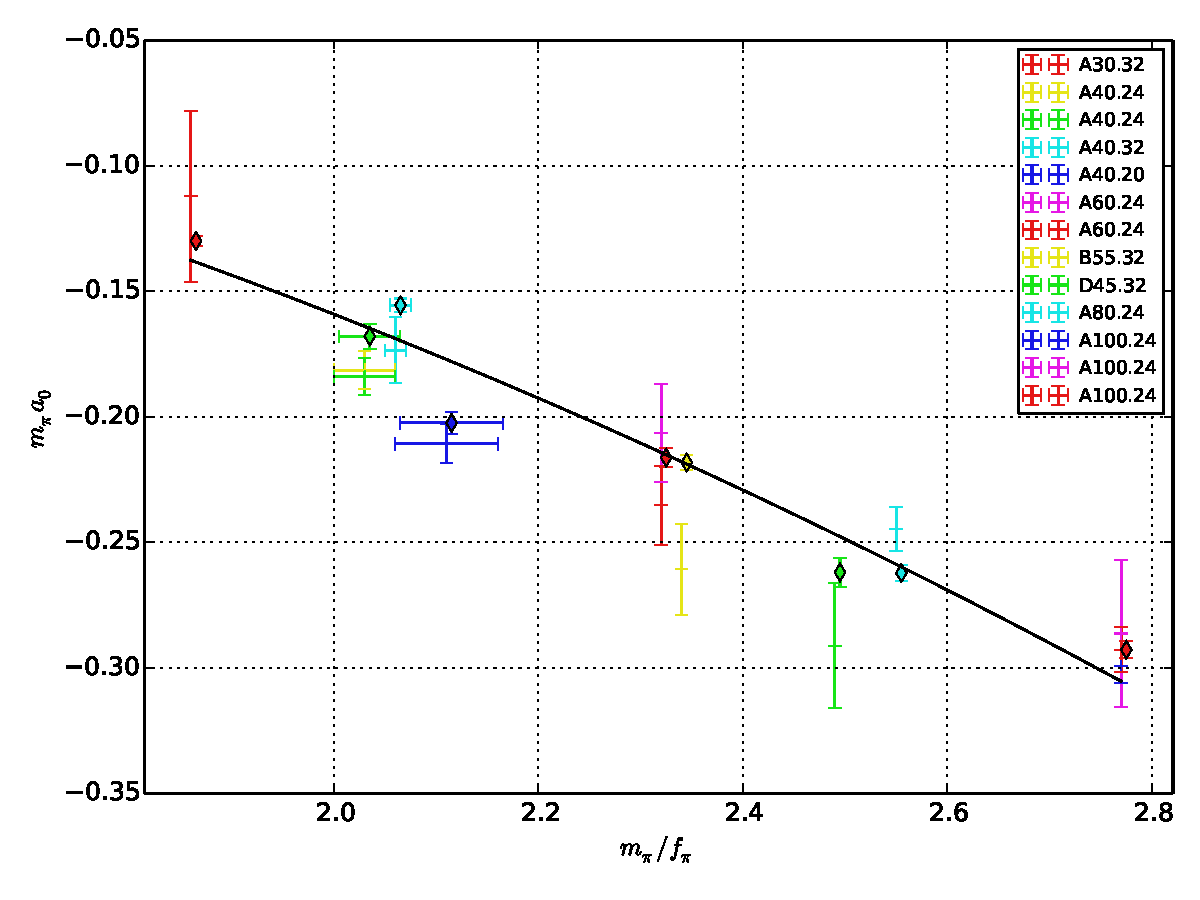
\includegraphics[width=\linewidth]{plots/result.pdf}
    \caption{%
        Results. Diamond data points are taken from draft paper.
    }
    \label{fig:result}
\end{figure}

\end{document}

% vim: spell spelllang=en tw=79
